\documentclass[11pt]{beamer}
\usepackage{graphicx}
\graphicspath{ {./Images/} }
\setbeamertemplate{caption}[numbered]
\usepackage{caption}
\usepackage{float}
\usepackage{hyperref}
\usepackage{multirow}
\setbeamersize{text margin left=0.5cm,text margin right=0.5cm}
\usepackage{multicol}
\usepackage{listings}
\usepackage{color}
\usepackage{fancyvrb}
\usepackage{booktabs}
\definecolor{dkgreen}{rgb}{0,0.6,0}
\definecolor{gray}{rgb}{0.5,0.5,0.5}
\definecolor{mauve}{rgb}{0.58,0,0.82}
\lstset{
  language=Java,
  aboveskip=3mm,
  belowskip=3mm,
  showstringspaces=false,
  columns=flexible,
  basicstyle={\small\ttfamily},
  numbers=none,
  frame=single,
  numberstyle=\tiny\color{gray},
  keywordstyle=\color{blue},
  commentstyle=\color{dkgreen},
  stringstyle=\color{mauve},
  breaklines=true,
  breakatwhitespace=true,
  tabsize=3,
  fancyvrb=true,
}

\makeatletter
\let\save@measuring@true\measuring@true
\def\measuring@true{%
  \save@measuring@true
  \def\beamer@sortzero##1{\beamer@ifnextcharospec{\beamer@sortzeroread{##1}}{}}%
  \def\beamer@sortzeroread##1<##2>{}%
  \def\beamer@finalnospec{}%
}
\makeatother

\mode<presentation> {
    \usetheme{Warsaw}
    \setbeamertemplate{footline}[page number]
    }

\definecolor{violet}{rgb}{0.54, 0.17, 0.89}
\newcommand{\red}[1]{\textcolor{red}{#1}}
\newcommand{\violet}[1]{\textcolor{violet}{#1}}
\newcommand{\green}[1]{\textcolor{green}{#1}}
\newcommand{\sol}{\textbf{Solution}: \pause \newline}

\title[Chapter 07 Notes]{Math 130: Introduction to Programming \\ Chapter 07: Introduction to Arrays \\ Lecture Notes}
\author{Jesús R. Pérez Cuarenta \\
\href{mailto:jperezcuarenta@swccd.edu}{jperezcuarenta@swccd.edu}
}
\date{}

\begin{document}
\begin{frame}
  \maketitle
\end{frame}

\begin{frame}
\frametitle{Overview}
    \begin{multicols}{2}
    \tableofcontents
    \end{multicols}
\end{frame}

\section{Introduction to Arrays}
\subsection{Introduction to Arrays}
\begin{frame}[fragile]{Introduction to Arrays}
    An \red{array} can \red{hold multiple values} of the \red{same data type} simultaneously. \\ \vspace{1em}

    Primitive variables are designed to hold one value at a time. \\ \vspace{1em}

    An array is an object that can store a group of values. \\ \vspace{1em}

    Creating and using an array is similar to creating and using any other type of object.

    \begin{lstlisting}
int[] numbers = new int[6];
float[] temperatures = new float[100];
char[] letters = new char[41];
long[] units = new long[50];
double[] sizes = new double[1200];
    \end{lstlisting}
\end{frame}

\begin{frame}[fragile]{Introduction to Arrays}
    An array's size declarator must be non-negative integer expression. \\ \vspace{1em}

    It is common practice to use a \textbf{final} variable as a size decorator. \\ \vspace{1em}

    \begin{lstlisting}
final int NUM_ELEMENTS = 6;
int[] numbers = new int[NUM_ELEMENTS];
    \end{lstlisting}

    Note: Once an array is created, its size cannot be changed.
\end{frame}

\begin{frame}[fragile]{Accessing Array Elements}
    A graphical representation of
    \begin{lstlisting}  
int[] numbers = new int[6];
    \end{lstlisting}
    is the following:
    \noindent 
    \begin{figure}[H]
    \centering
    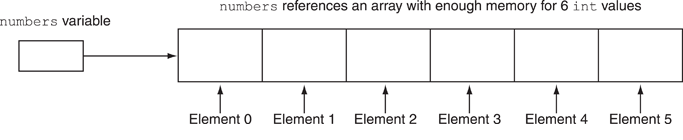
\includegraphics[scale=0.7]{Images/chapter07_arrayExample.png}
    \end{figure}
    The elements in the array may be accessed and used as individual variables.  \\ \vspace{1em}
    Each element is assigned a number known as a \textit{subscript}. \\ \vspace{1em}
\end{frame}

\begin{frame}[fragile]{Accessing Array Elements}
    Each element in the \textbf{numbers} array, when accessed by its subscript, can be used as an \textbf{int} variable.
    \begin{lstlisting}
int[] numbers = new int[6];
numbers[0] = 20;
numbers[3] = 30;
    \end{lstlisting}
    \noindent 
    \begin{figure}[H]
    \centering
    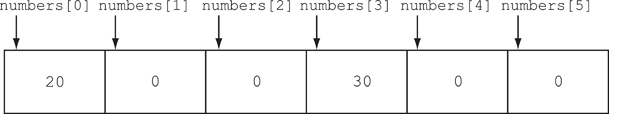
\includegraphics[scale=0.7]{Images/chapter07_accessingArray.png}
    \end{figure}
Note: By default, Java initializes array elements to 0.
\end{frame}

\begin{frame}[fragile]{Accessing Array Elements}
Here is an example where we iterate over the subscripts of an array, a very common practice when programming.
    \begin{lstlisting}
public static void main(String[] args) {
    Scanner kb = new Scanner(System.in);
    final int ARRAY_SIZE = 3;
    int[] numbers = new int[ARRAY_SIZE];
    for (int idx = 0; idx < ARRAY_SIZE; idx++) {
        System.out.println("Enter a number: ");
        numbers[idx] = kb.nextInt();
        }
    kb.close();
    }
    \end{lstlisting}
\end{frame}

\begin{frame}[fragile]{Java Performs Bounds Checking}
    You cannot use a subscript outside the range of valid subscripts for an array.
    \begin{lstlisting}
int[] values = new int[3];
for (int index = 0; index < 4; index++) {
    values[index] = 10; // error when index == 3
    }
    \end{lstlisting}
\end{frame}

\begin{frame}[fragile]{Array Initialization}
    There are other ways to initialize an array with elements of type \textbf{int}.
    \begin{lstlisting}
int[] days = {31, 28, 31, 30, 31, 30, 31, 31, 30, 31, 30, 31};
    \end{lstlisting}
    In this example,
\begin{itemize}
    \item The first value, 31, is stored in \textbf{days[0]}
    \item The second value, 28, is stored in \textbf{days[1]}
    \item and so on ... 
\end{itemize}
    The Java compiler determines the size of the array by the number of items in the initialization list.
\end{frame}

\subsection{Processing Array Elements}
\begin{frame}[fragile]
    \frametitle{Processing Array Elements}
    Individual array elements are processed like any other type of variable.
    \begin{lstlisting}
grossPay = hours[3] * payRate;
    \end{lstlisting}
    Examples of pre-increment and post-increment operations on array elements:
    \begin{lstlisting}
int[] score = {7, 8, 9, 10, 11};
++score[2]; // Pre-increment operation
score[4]++; // Post-increment operation
    \end{lstlisting}
    When using increment and decrement operators, be careful not to use the operator on the subscript when you intend to use it on the array element:
    \begin{lstlisting}
amount[count--];
    \end{lstlisting}
\end{frame}

\begin{frame}[fragile]
    \frametitle{Array Length}
    Each array in Java has a public field named \texttt{length}. This field contains the number of elements in the array.
    \begin{lstlisting}[basicstyle=\ttfamily\footnotesize]
double[] temperatures = new double[25];
    \end{lstlisting}
    Because the \texttt{temperatures} array has 25 elements, the following statement would assign 25 to the variable \texttt{size}:
    \begin{lstlisting}[basicstyle=\ttfamily\footnotesize]
size = temperatures.length;
    \end{lstlisting}
    The \texttt{length} field can be useful when processing the entire contents of an array.
    \begin{lstlisting}[basicstyle=\ttfamily\footnotesize]
for (int idx = 0; idx < temperatures.length; idx++) {
    System.out.println(temperatures[idx]);
    }
    \end{lstlisting}
\end{frame}

\begin{frame}[fragile]
    \frametitle{The Enhanced for Loop}
    Java provides a specialized version of the \texttt{for} loop known as the enhanced \texttt{for} loop.
    \begin{lstlisting}[basicstyle=\ttfamily\footnotesize]
for (dataType elementVariable : array) {
    statement;
    }
    \end{lstlisting}
    For example, with the following array declaration:
    \begin{lstlisting}[basicstyle=\ttfamily\footnotesize]
int[] numbers = {3, 6, 9};
    \end{lstlisting}
    You can use the enhanced \texttt{for} loop to display the contents of the \texttt{numbers} array:
    \begin{lstlisting}[basicstyle=\ttfamily\footnotesize]
for (int val : numbers) {
    System.out.println(val);
    }
    \end{lstlisting}
\end{frame}

\begin{frame}[fragile]
    \frametitle{The Enhanced for Loop versus the Traditional for Loop}
    There are circumstances in which the enhanced \texttt{for} loop is not adequate:
    \begin{itemize}
        \item If you need to change the contents of an array element.
        \item If you need to work through the array elements in reverse order.
        \item If you need to access some of the array elements, but not all of them.
        \item If you need to work with two or more arrays within the loop.
        \item If you need to refer to the subscript number of a particular element.
    \end{itemize}
    In any of these circumstances, you should use the traditional \texttt{for} loop to process the array.
\end{frame}

\begin{frame}[fragile]
    \frametitle{Reassigning Array Reference Variables}
    It is possible to reassign an array reference variable to a different array.
    \begin{lstlisting}
// Create an array referenced by the numbers variable.
int[] numbers = new int[10];
// Reassign numbers to a new array.
numbers = new int[5];
    \end{lstlisting}
    The first statement creates a ten-element integer array and assigns its address to the \texttt{numbers} variable. \\ \vspace{1em} 
    The second statement allocates a five-element integer array and assigns its address to the \texttt{numbers} variable. \\ \vspace{1em} 
    The ten-element array is no longer referenced and cannot be accessed.
\end{frame}

\begin{frame}[fragile]
    \frametitle{Copying Arrays}
    Because an array and the reference variable are separate entities, you cannot copy an array by merely assigning one array reference variable to another. \\ \vspace{1em} 
    Instead, to copy an array, you need to copy the individual elements from one array to another. \\ \vspace{1em} 
    Usually, this is best done with a loop.
    \begin{lstlisting}
int[] firstArray = {5, 10, 15, 20, 25};
int[] secondArray = new int[5];
for (int idx = 0; idx < firstArray.length; idx++) {
    secondArray[idx] = firstArray[idx];
    }
    \end{lstlisting}
    The loop in this code copies each element of \texttt{firstArray} to the corresponding element of \texttt{secondArray}.
\end{frame}

\section{Arrays and Methods}
\subsection{Passing Arrays as Arguments to Methods}
\begin{frame}[fragile]
    \frametitle{Passing Arrays as Arguments to Methods}
    An array can be passed as an argument to a method. \\ \vspace{1em}
    To pass an array, you pass the value in the variable that references the array.
    \begin{lstlisting}
public static void main(String[] args) {
    int[] numbers = {3, 6, 9, 12, 15};
    showArray(numbers);
    }
public static void showArray(int[] array) {
    for (int idx = 0; idx < array.length; i++) {
        System.out.print(array[idx] + " ");
        }
    }
    \end{lstlisting}
    When an entire array is passed into a method, it is passed just as an object is passed. The method has direct access to the original array.
\end{frame}

\begin{frame}[fragile]
    \frametitle{Using Methods to Process Arrays}
    When a single element of an array is passed to a method, it is handled like any other variable. \\ \vspace{1em}
    The method accepts an argument and processes it as needed.
    \begin{lstlisting}
public static void main(String[] args) {
    int[] numbers = {3, 6, 9, 12, 15};
    for (int num : numbers) {
        showValue(num);
        }
    }
public static void showValue(int n) {
    System.out.println(n);
    }
    \end{lstlisting}
\end{frame}

\subsection{Useful Array Algorithms and Operations}
\begin{frame}[fragile]
    \frametitle{Comparing Arrays}
    You cannot copy an array by simply assigning its reference variable to another array's reference variable. The `==` operator cannot be used to compare two array reference variables.
    \begin{lstlisting}
int[] firstArray = {5, 10, 15, 20, 25};
int[] secondArray = {5, 10, 15, 20, 25};
if (firstArray == secondArray) {
    System.out.println("The arrays are the same.");
    }
else {
    System.out.println("The arrays are not the same.");
    }
    \end{lstlisting}
    When using `==` with reference variables, it compares memory addresses, not contents.
\end{frame}

\begin{frame}[fragile]
    \frametitle{Comparing Array Contents}
    To compare the contents of two arrays, you must compare the elements of the arrays.
    \begin{lstlisting}[basicstyle=\ttfamily\footnotesize]
int[] firstArray = {2, 4, 6, 8, 10};
int[] secondArray = {2, 4, 6, 8, 10};
boolean arraysEqual = true;
int index = 0;
if (firstArray.length != secondArray.length) {
    arraysEqual = false;
    }
while (arraysEqual && index < firstArray.length) {
    if (firstArray[index] != secondArray[index]) {
        arraysEqual = false;
        }
    index++;
    }
if (arraysEqual)
    System.out.println("The arrays are equal.");
    \end{lstlisting}
\end{frame}

\begin{frame}[fragile]
    \frametitle{Summing the Values in a Numeric Array}
    To sum the values in an array, you must use a loop with an accumulator variable.
    \begin{lstlisting}
int[] units = new int[25];
int total = 0;
for (int idx = 0; idx < units.length; idx++) {
    total += units[idx];
    }
    \end{lstlisting}
\end{frame}

\begin{frame}[fragile]
    \frametitle{Getting the Average of the Values in a Numeric Array}
    Calculating the average of values in an array involves two steps: summing the values and then dividing the sum by the number of elements.
    \begin{lstlisting}
double[] scores = new double[10];
double total = 0;
double average;
for (int index = 0; index < scores.length; index++) {
    total += scores[index];
    }
average = total / scores.length;
    \end{lstlisting}
\end{frame}

\begin{frame}[fragile]
    \frametitle{Finding the Highest and Lowest Values in a Numeric Array}
    Finding the highest value:
    \begin{lstlisting}
int[] numbers = new int[50];
int highest = numbers[0];
for (int index = 1; index < numbers.length; index++) {
    if (numbers[index] > highest) {
        highest = numbers[index];
        }
    }
    \end{lstlisting}
\end{frame}

\begin{frame}[fragile]
    \frametitle{Finding the Highest and Lowest Values (Contd.)}
    Finding the lowest value:
    \begin{lstlisting}
int[] numbers = new int[50];
int lowest = numbers[0];
for (int index = 1; index < numbers.length; index++) {
    if (numbers[index] < lowest) {
        lowest = numbers[index];
        }
    }
    \end{lstlisting}
\end{frame}

\begin{frame}[fragile]
    \frametitle{Working with Arrays and Files}
    You can use a loop to write each element of the array to the file.
    \begin{lstlisting}
int[] numbers = {10, 20, 30, 40, 50};
PrintWriter outputFile = new PrintWriter("Values.txt");
for (int idx = 0; idx < numbers.length; idx++) {
    outputFile.println(numbers[index]);
    }
outputFile.close();
    \end{lstlisting}
\end{frame}

\begin{frame}[fragile]
    \frametitle{Reading Data from Files into Arrays}
    To read data from a file into an array, you can open the file and use a loop to read values from the file and store them in the array.
    \begin{lstlisting}
final int SIZE = 5;
int[] numbers = new int[SIZE];
int idx = 0;
File file = new File("Values.txt");
Scanner inputFile = new Scanner(file);
while (inputFile.hasNext() && idx < numbers.length) {
    numbers[idx] = inputFile.nextInt();
    idx++;
    }
inputFile.close();
    \end{lstlisting}
\end{frame}

\subsection{Returning Arrays from Methods}
\begin{frame}[fragile]
    \frametitle{Returning Arrays from Methods}
    In addition to accepting arrays as arguments, methods may also return arrays.
    \begin{lstlisting}
public static double[] getArray() {
    double[] array = {1.2, 2.3, 4.5, 6.7, 8.9};
    return array;
    }
    \end{lstlisting}
    The \texttt{getArray} method returns an array of \texttt{double}s. \\ \vspace{1em}
    Notice that the return type listed in the method header is \texttt{double[]}. \\ \vspace{1em} 
    The method header indicates that the method returns a reference to a \texttt{double} array.
\end{frame}

\begin{frame}[fragile]
    \frametitle{Using the Returned Array}
    Here is a more complete example.
    \begin{lstlisting}
public static void main(String[] args) {
    double[] values = getArray();
    for (int idx = 0; idx < values.length; idx++) {
        System.out.println(values[idx]);
        }
public static double[] getArray() {
    double[] array = {1.2, 2.3, 4.5, 6.7, 8.9};
    return array;
    }
    \end{lstlisting}
    The code assigns the array returned by the \texttt{getArray} method to the \texttt{values} variable and then displays the values in the array using a \texttt{for} loop.
\end{frame}

\section{Arrays of Objects and Sequential Search Algorithm}
\subsection{String Arrays}
\begin{frame}[fragile]
    \frametitle{String Arrays}
    An array of String objects may be created. If the array is uninitialized, each String in the array must be created individually.
    \begin{lstlisting}
String[] names = {"Bill", "Susan", "Steven", "Jean"};
    \end{lstlisting}
    To use a String object, you must have a reference to it, so an array of String objects is really an array of references to String objects.
    \begin{lstlisting}
final int SIZE = 4;
String[] names = new String[SIZE];
    \end{lstlisting}
\end{frame}

\begin{frame}
{String Arrays}
    \noindent 
    \begin{figure}[H]
    \centering
    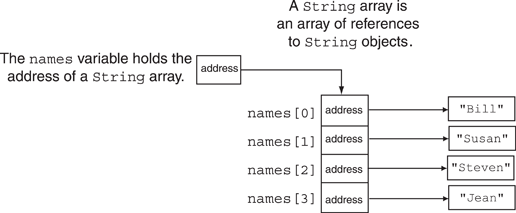
\includegraphics[scale=0.8]{Images/chapter07_section06_fig14.png}
    \end{figure}    
\end{frame}

\begin{frame}[fragile]
    \frametitle{Working with Uninitialized String Arrays}
    When you create an uninitialized array of String objects, you must assign a value to each element in the array that you intend to use.
    \begin{lstlisting}
final int SIZE = 4;
String[] names = new String[SIZE];
names[0] = "Bill";
names[1] = "Susan";
names[2] = "Steven";
names[3] = "Jean";
    \end{lstlisting}
\end{frame}

\begin{frame}[fragile]
    \frametitle{Calling String Methods from an Array Element}
    Because each element of a String array is a String object, you can use an element to call a String method.
    \begin{lstlisting}
System.out.println(names[0].toUpperCase());
    \end{lstlisting}
    The following code uses element 3 of the names array to call the charAt method.
    \begin{lstlisting}
char letter;
letter = names[3].charAt(0);
    \end{lstlisting}
\end{frame}

\begin{frame}[fragile]
    \frametitle{Warning}
    Arrays have a \red{field} named \red{length}. \\ \vspace{1em}
    String objects have a \violet{method} named \violet{length}. \\ \vspace{1em}
    Do not confuse the two when working with String arrays.
    \begin{lstlisting}
for (int idx = 0; idx < names.length; idx++) {
    System.out.println(names[idx].length());
    }
    \end{lstlisting}
\end{frame}

\subsection{Arrays of Objects}
\begin{frame}[fragile]
    \frametitle{Arrays of Objects}
    You may create arrays of objects that are instances of classes that you have written.
    \begin{lstlisting}
final int NUM_ACCOUNTS = 5;
BankAccount[] accounts = new BankAccount[NUM_ACCOUNTS];
    \end{lstlisting}
    Each element in this array is a reference variable, initialized with the value `null`. You must individually create the objects that each element will reference.
    \begin{lstlisting}
for (int idx = 0; idx < accounts.length; idx++)
    accounts[idx] = new BankAccount();
    \end{lstlisting}
\end{frame}

\begin{frame}[fragile]{Arrays of Objects}
Here is a graphical representation of
\begin{lstlisting}
BankAccount[] accounts = new BankAccount[5];
\end{lstlisting}
    \noindent 
    \begin{figure}[H]
    \centering
    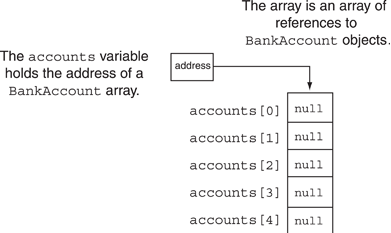
\includegraphics[scale=0.8]{Images/chapter07_section06_fig16.png}
    \end{figure}   
\end{frame}

\begin{frame}[fragile]{Arrays of Objects}
Similarly, here is a graphical representation of
\begin{lstlisting}
for (int idx = 0; idx < accounts.length; idx++)
    accounts[idx] = new BankAccount();
\end{lstlisting}
    \noindent 
    \begin{figure}[H]
    \centering
    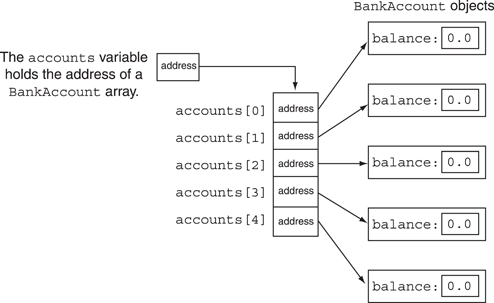
\includegraphics[scale=0.6]{Images/chapter07_section06_fig17.png}
    \end{figure}   
\end{frame}

\begin{frame}[fragile]
    \frametitle{Accessing Objects in the Array}
    Objects in an array are accessed with subscripts, just like any other data type in an array.
    \begin{lstlisting}
accounts[2].setBalance(2500.0);
accounts[2].withdraw(500.0);
    \end{lstlisting}
    After this code executes, the `accounts[2]` element references a `BankAccount` object.
\end{frame}

\subsection{Sequential Search Algorithm}
\begin{frame}[fragile]
    \frametitle{Sequential Search Algorithm}

    A search algorithm is a method of locating a specific item in a larger collection of data. The sequential search is a simple technique for searching the contents of an array.

    \begin{lstlisting}[basicstyle=\ttfamily\footnotesize]
public static int sequentialSearch(int[] array, int value) {
    int index = 0;
    int element = -1;
    boolean found = false;
    while (!found && index < array.length) {
        if (array[index] == value) {
            found = true;
            element = index;
            }
        index++;
        }
    return element;
    }
    \end{lstlisting}
\end{frame}

\begin{frame}[fragile]
    \frametitle{Example of Sequential Search}
    The `SearchArray` program searches for the value 100 in an array.
    \begin{lstlisting}[basicstyle=\ttfamily\footnotesize]
// SearchArray.java
int[] tests = {87, 75, 98, 100, 82};
int results;
// Search the array for the value 100.
results = sequentialSearch(tests, 100);
// Determine whether 100 was found.
if (results == -1) {
    System.out.println("You did not earn 100 on any test.");
    } 
else {
    System.out.println("You earned 100 on test " + (results + 1));
    }
    \end{lstlisting}
\end{frame}

\section{Multi-Dimensional Arrays, More Search Algorithms, ArrayList}
\subsection{Two-Dimensional Arrays}
\begin{frame}[fragile]
\frametitle{Introduction to Two-Dimensional Arrays}
    A two-dimensional array is an array of arrays, providing a way to represent data with rows and columns. \\ \vspace{1em}
    To declare a two-dimensional array, use two sets of brackets: one for rows and one for columns.
    \begin{lstlisting}[language=Java]
double[][] scores = new double[3][4];
    \end{lstlisting}
    Access elements in a two-dimensional array using two subscripts: one for row and one for column.
    \begin{lstlisting}
scores[2][1] = 95;
    \end{lstlisting}
\end{frame}

\begin{frame}{Introduction to Two-Dimensional Arrays}
    \noindent 
    \begin{figure}[H]
    \centering
    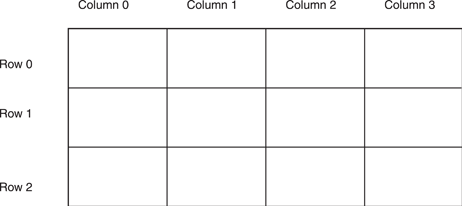
\includegraphics[scale=0.6]{Images/chapter07_section09_fig18.png}
    \end{figure}   
\end{frame}

\begin{frame}[fragile]
\frametitle{Iterating Through a 2D Array}
Use nested loops to process all elements in a 2D array.
\begin{lstlisting}[language=Java]
for (int row = 0; row < scores.length; row++) {
    for (int col = 0; col < scores[row].length; col++) {
        // Process scores[row][col]
        }
    }
\end{lstlisting}
\end{frame}

\begin{frame}{Iterating Through a 2D Array}
    \noindent 
    \begin{figure}[H]
    \centering
    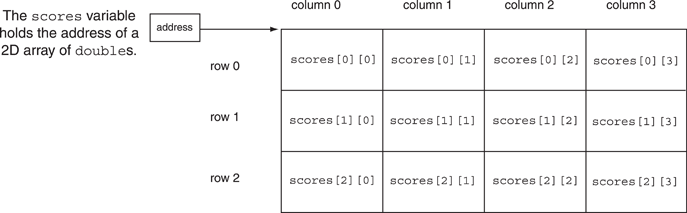
\includegraphics[scale=0.6]{Images/chapter07_section09_fig20.png}
    \end{figure}       
\end{frame}

\begin{frame}[fragile]
\frametitle{Summing Elements in a 2D Array}

To sum all elements in a 2D array, use nested loops and an accumulator.

\begin{lstlisting}[language=Java]
int total = 0;
for (int row = 0; row < scores.length; row++) {
    for (int col = 0; col < scores[row].length; col++) {
        total += scores[row][col];
    }
}
\end{lstlisting}

\end{frame}

\begin{frame}[fragile]
\frametitle{Passing 2D Arrays to Methods}
\framesubtitle{Method Parameter}

When passing a 2D array to a method, the parameter should be declared as a reference to a 2D array.

\begin{lstlisting}[language=Java]
private static void processArray(int[][] array) {
    // Process the array
}
\end{lstlisting}

\end{frame}

\begin{frame}[fragile]
\frametitle{Ragged Arrays}
\framesubtitle{Arrays with Varying Row Lengths}

Ragged arrays have rows of different lengths. You can create them using:

\begin{lstlisting}[language=Java]
int[][] ragged = new int[4][];
ragged[0] = new int[3];
ragged[1] = new int[4];
ragged[2] = new int[5];
ragged[3] = new int[6];
\end{lstlisting}
\end{frame}

\subsection{Introduction to Arrays with Multiple Dimensions}
\begin{frame}[fragile]
\frametitle{Declaring Multi-Dimensional Arrays}
\framesubtitle{Creating Complex Structures}

You can declare arrays with virtually any number of dimensions.
\begin{lstlisting}[language=Java]
double[][][] seats = new double[3][5][8];
\end{lstlisting}
As an example, this array consists of three sets of five rows, each with eight elements, such as seat prices.
\end{frame}

\begin{frame}[fragile]
\frametitle{Applications of Multi-Dimensional Arrays}
\framesubtitle{Beyond Three Dimensions}

While three-dimensional arrays are common, you can use arrays with more dimensions to tackle complex problems.

\begin{lstlisting}[language=Java]
// Example of a four-dimensional array
int[][][][][] warehouse = new int[3][4][5][6][10];
\end{lstlisting}
In some cases, additional dimensions represent different aspects of the data.
\end{frame}

\subsection{Selection Sort and the Binary Search Algorithm}
\begin{frame}{Selection Sort and the Binary Search Algorithm}
    A sorting algorithm is used to arrange data into some order. \\ \vspace{1em}

    A search algorithm is a method of locating a specific item in a larger collection of data. \\ \vspace{1em}
    
    The selection sort and the binary search are popular sorting and searching algorithms.
\end{frame}

\begin{frame}{Selection Sort Algorithm}
    A sorting algorithm is a technique for scanning through an array and rearranging its contents in some specific order. \\ \vspace{1em} 
    The selection sort works like this: The smallest value in the array is located and moved to element 0. \\ \vspace{1em} 
    Then the next smallest value is located and moved to element 1. \\ \vspace{1em} 
    This process continues until all of the elements have been placed in their proper order.
\end{frame}

\begin{frame}{Selection Sort Algorithm}
    Initially, the array may look like the following.
    \noindent 
    \begin{figure}[H]
    \centering
    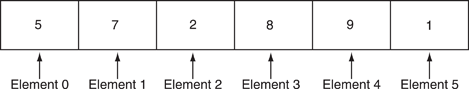
\includegraphics[scale=0.5]{Images/chapter07_section11_SortAlgorithm.png}
    \end{figure}
    After the first iteration,
    \noindent 
    \begin{figure}[H]
    \centering
    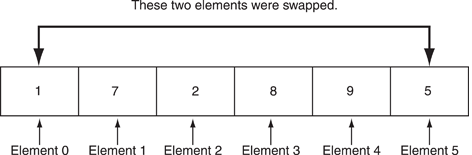
\includegraphics[scale=0.5]{Images/chapter07_section11_SortAlgorithm02.png}
    \end{figure}
    After the second iteration,
    \noindent 
    \begin{figure}[H]
    \centering
    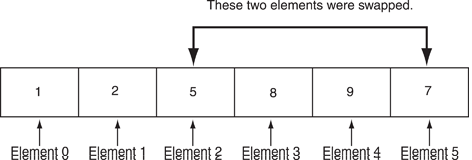
\includegraphics[scale=0.5]{Images/chapter07_section11_SortAlgorithm03.png}
    \end{figure}
\end{frame}

\begin{frame}[fragile]
{Selection Sort Algorithm}
    \begin{lstlisting}[basicstyle=\ttfamily\footnotesize]
public static void selectionSort(int[] array) {
    int startScan, index, minIndex, minValue;
    for (startScan = 0; startScan < array.length - 1; startScan++) {
        minIndex = startScan;
        minValue = array[startScan];
        for(index = startScan + 1; index < array.length; index++) {
            if (array[index] < minValue) {
                minValue = array[index];
                minIndex = index; 
                }
            }
        array[minIndex] = array[startScan];
        array[startScan] = minValue;
        }
    \end{lstlisting}
\end{frame}

\begin{frame}[fragile]
\title{Binary Search Algorithm}
    The sequential search algorithm is simple but inefficient. \\ \vspace{1em}
    The sequential search should not be used on large arrays if speed is important (\red{why?}). \\ \vspace{1em}
    We will now study the binary search but we need to assume the array is sorted in ascending order.
    \noindent 
    \begin{figure}[H]
    \centering
    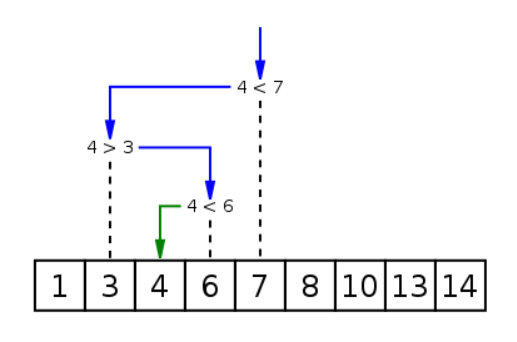
\includegraphics[scale=0.6]{Images/chapter07_section11_BinarySearch01.png}
    \end{figure}
\end{frame}

\begin{frame}[fragile]
{Binary Search Algorithm}
    \begin{lstlisting}[basicstyle=\ttfamily\footnotesize]
public static int binarySearch(int[] array, int value) {
    int first, last, middle, position;
    boolean found;
    first = 0; last = array.length - 1; position = -1; found = false;
    while (!found && first <= last) {
        middle = (first + last) / 2;
        if (array[middle] == value) {
            found = true;
            position = middle;
            }
        else if (array[middle] > value)
            last = middle - 1;
        else
            first = middle + 1;
        }
    return position;
    }
    \end{lstlisting}
\end{frame}


\begin{frame}[fragile]
{Command-Line Arguments and Variable-Length Argument Lists}
    When you invoke a Java program from the operating system command line, you can specify arguments that are passed into the main method of the program. \\ \vspace{1em} 
    In addition, you can write a method that takes a variable number of arguments. \\ \vspace{1em} 
    When the method runs, it can determine the number of arguments that were passed to it and act accordingly.
\end{frame}

\begin{frame}[fragile]
{Command-Line Arguments}
    Every program you have seen in this book and every program you have written uses a static main method with a header that looks like this:
    \begin{lstlisting}
public static void main(String[] args)
    \end{lstlisting}
    Inside the parentheses of the method header is the declaration of a parameter named \texttt{args}. This parameter is an array name. \\ \vspace{1em}
    As its declaration indicates, it is used to reference an array of Strings. \\ \vspace{1em}
    The array that is passed into the \texttt{args} parameter comes from the operating system command line.
\end{frame}

\begin{frame}[fragile]
{Command-Line Arguments}
Take the following Java file as an example.
    \begin{lstlisting}
package week10;
public class CommandLineDemo {
	public static void main(String[] args) {
		for (int idx = 0; idx < args.length; idx++) {
			System.out.println(args[idx]);
			}
		}
	}
    \end{lstlisting}
\end{frame}

\begin{frame}[fragile]
{Command-Line Arguments}
We can run the program from the Command Prompt in Windows.
    \noindent 
    \begin{figure}[H]
    \centering
    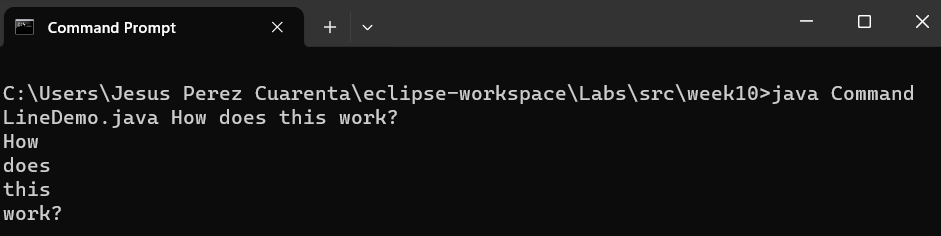
\includegraphics[scale=0.6]{Images/chapter07_section12_cmdArgs.png}
    \end{figure}
    Note that the word `How` is passed into \texttt{args[0]}, `does` is passed into \texttt{args[1]}, `this` is passed into \texttt{args[2]}, and `work? ` is passed into \texttt{args[3]}.
\end{frame}

\begin{frame}[fragile]
{Variable-Length Argument Lists}
    Java provides a mechanism known as variable-length argument lists, which makes it possible to write a method that takes a \red{variable number of arguments}. \\ \vspace{1em}
    For example, suppose we need to write a method named sum that can accept any number of int values and then return the sum of those values.
    \begin{lstlisting}
int firstVal, secondVal, thirdVal, fourthVal;
firstVal = 5, secondVal = 3; thirdVal = 10; fourthVal = 20;
// we want both calls to _sum_ to be valid
result = sum(10, 20);
result = sum(firstVal, secondVal, thirdVal, fourthVal);
    \end{lstlisting}
\end{frame}

\begin{frame}[fragile]
{Variable-Length Argument Lists}
    To achieve a multi-purpose method, we can write the following.
    \begin{lstlisting}[basicstyle=\ttfamily\footnotesize]
public static void main(String[] args) {
    int output;
    int firstVal, secondVal, thirdVal, fourthVal;
    firstVal = 5; secondVal = 3; thirdVal = 10; fourthVal = 20;
    output = sum(10, 20);
    System.out.printf("The output is %d\n", output);
    output = sum(firstVal, secondVal, thirdVal, fourthVal);
    System.out.printf("The output is %d\n", output);
    }
public static int sum(int... numbers) {
    int total = 0;
    for (int val : numbers)
        total += val;
    return total;
    }
    \end{lstlisting}
\end{frame}

\begin{frame}[fragile]
{Variable-Length Argument Lists}
    The previous slide showcases a special type of parameter (note the uses of three periods) known as \texttt{vararg parameter}.
    \begin{lstlisting}
public static int sum(int... numbers)
    \end{lstlisting}
    We have that \texttt{vararg} parameters are actually arrays. \\ \vspace{1em} 
    All of the arguments that are passed to the \texttt{sum} method are stored in the elements of the \texttt{numbers} array.
\end{frame}

\subsection{The \texttt{ArrayList} Class}
\begin{frame}[fragile]
{The \texttt{ArrayList} Class}
    \texttt{ArrayList} is a class similar to that of an array and it allows you to store objects. \\ \vspace{1em}
    Unlike an array, an \texttt{ArrayList} object’s size is \red{automatically adjusted} to accommodate the number of items being stored in it. \\ \vspace{1em}
    \begin{lstlisting}[basicstyle=\ttfamily\footnotesize]
import java.util.*;
public class ArrayListDemo {
	public static void main(String[] args) {
		// create obj and store address
		ArrayList<String> nameList = new ArrayList<String>();
		// add references to String objects
		nameList.add("James");
		nameList.add("Catherine");
		nameList.add("Bill");
		}
	}
    \end{lstlisting}    
\end{frame}

\begin{frame}[fragile]
{The \texttt{ArrayList} Class}
    Some useful ArrayList methods are \texttt{size}, \texttt{get}, \texttt{remove}, and \texttt{add}.
    \begin{lstlisting}[basicstyle=\ttfamily\footnotesize]
// Assume nameList = {"James", "Catherine", "Bill"};
System.out.println(
    "The arrayList has "
    + nameList.size()
    + " objects stored in it"
    );
System.out.println(nameList.get(1)); // "Catherine"
nameList.remove(1);
System.out.println(nameList.get(1)); // "Bill"
nameList.add(1, "Catherine");
System.out.println(nameList.get(1)); // "Catherine"
nameList.set(1, "Jennifer");
System.out.println(nameList.get(1)); // "Jennifer"
    \end{lstlisting}
\end{frame}

\begin{frame}[fragile]
{\texttt{ArrayList} Capacity}
    An \texttt{ArrayList} object has a capacity. \\ \vspace{1em}
    The capacity defines the number of items the object can store without having to increase its size. \\ \vspace{1em}
    When an \texttt{ArrayList} object is created using the no-arg constructor, it has an initial capacity of 10 items. \\ \vspace{1em}
    You can specify a different starting capacity:
    \begin{lstlisting}
ArrayList<String> someList = new ArrayList<String>(100);
    \end{lstlisting}
    
\end{frame}
\end{document}

